% ------------------------------------------------------------------------------
% TYPO3 CMS 8.4 - What's New - Chapter "Backend User Interface" (German Version)
%
% @author	Michael Schams and Patrick Lobacher
% @license	Creative Commons BY-NC-SA 3.0
% @link		http://typo3.org/download/release-notes/whats-new/
% @language	German
% ------------------------------------------------------------------------------
% LTXE-CHAPTER-UID:		07b25346-95b1df21-a6ebe09a-49f53f41
% LTXE-CHAPTER-NAME:	Backend User Interface
% ------------------------------------------------------------------------------

\section{Backend User Interface}
\begin{frame}[fragile]
	\frametitle{Backend User Interface}

	\begin{center}\huge{Kapitel 1:}\end{center}
	\begin{center}\huge{\color{typo3darkgrey}\textbf{Backend User Interface}}\end{center}

\end{frame}

% ------------------------------------------------------------------------------
% LTXE-SLIDE-START
% LTXE-SLIDE-UID:		03a5eae6-03db4728-9c62a0ec-835d205f
% LTXE-SLIDE-ORIGIN:	75977160-b74e3317-0f697728-71b501d1 English
% LTXE-SLIDE-TITLE:		Mobile Responsive TYPO3 Backend
% ------------------------------------------------------------------------------

\begin{frame}[fragile]
	\frametitle{Backend User Interface}
	\framesubtitle{Mobiles Responsiv TYPO3 Backend}

	Das TYPO3 Backend ist nun komplett \textbf{mobile responsive}.

	\begin{figure}
		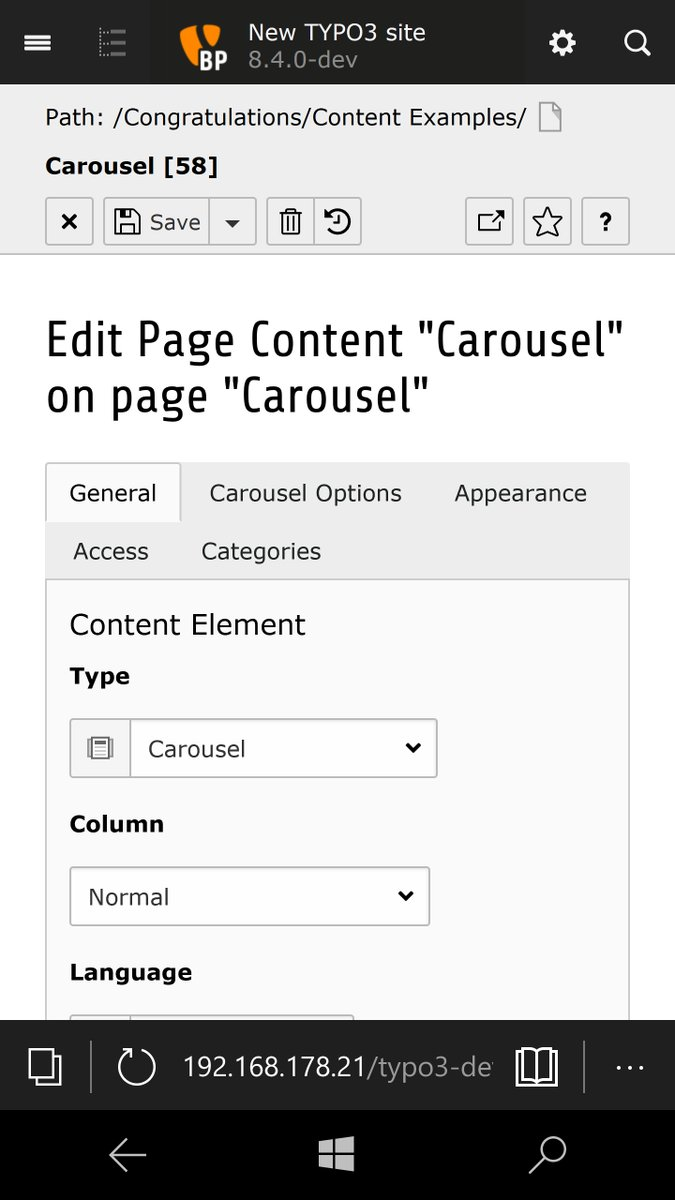
\includegraphics[width=0.25\linewidth]{BackendUserInterface/mobile-responsive-backend.jpg}
	\end{figure}

\end{frame}

% ------------------------------------------------------------------------------
% LTXE-SLIDE-START
% LTXE-SLIDE-UID:		8e42fc4f-2af7f825-dac9305c-ead95166
% LTXE-SLIDE-ORIGIN:	f6668b2d-8932a470-5b9c024c-e4e9f53a English
% LTXE-SLIDE-TITLE:		Install Tool: Upgrade Analysis
% ------------------------------------------------------------------------------

\begin{frame}[fragile]
	\frametitle{Backend User Interface}
	\framesubtitle{Install Tool: Upgrade Analyse}

	TYPO3 Versions-Upgrades werden nun mit dem neuen  \textbf{Upgrade Analysis} Tool im Install Tool vereinfacht (finden/filtern von dokumentierten Änderungen zwischen Versionen).

	\begin{figure}
		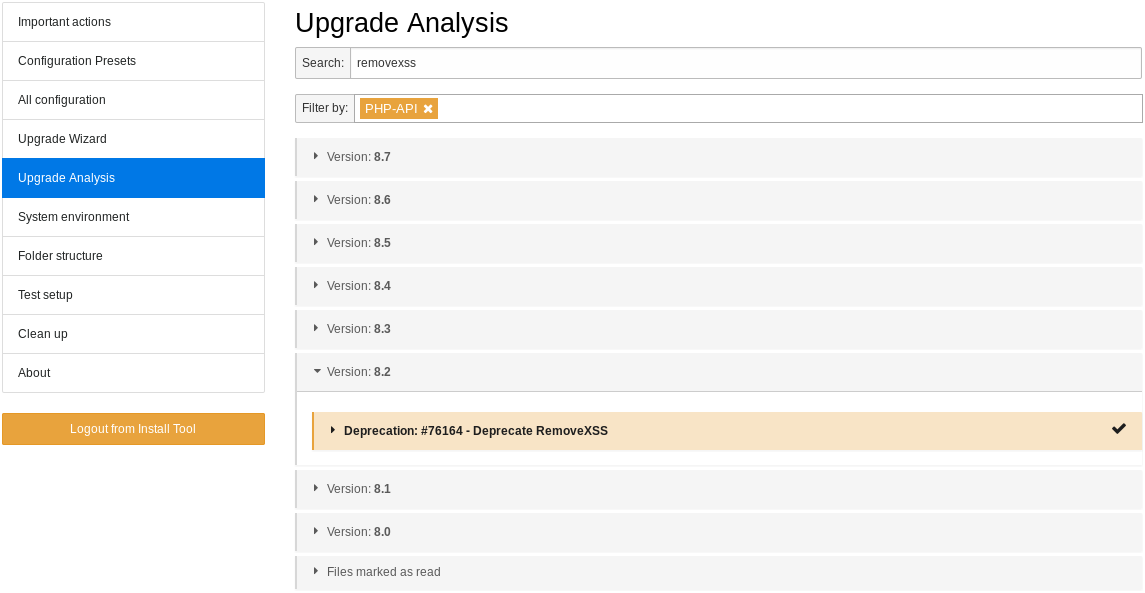
\includegraphics[width=0.45\linewidth]{BackendUserInterface/install-tool-upgrade-analysis.png}
	\end{figure}

\end{frame}

% ------------------------------------------------------------------------------
% LTXE-SLIDE-START
% LTXE-SLIDE-UID:		6e7f592a-0b16c696-23687e63-76cf36fa
% LTXE-SLIDE-ORIGIN:	9702aaf4-f02bbc35-67902b2e-42855506 English
% LTXE-SLIDE-TITLE:		Install Tool: Upgrade Analysis
% LTXE-SLIDE-REFERENCE:	#78222: Dump Class Loading Information UI in Install Tool
% ------------------------------------------------------------------------------

\begin{frame}[fragile]
	\frametitle{Backend User Interface}
	\framesubtitle{Install Tool: Dump Autoload Information}

	Es gibt nun eine Option im Installtool, um die Autoload Informationen neu zu erstellen.

	\begin{figure}
		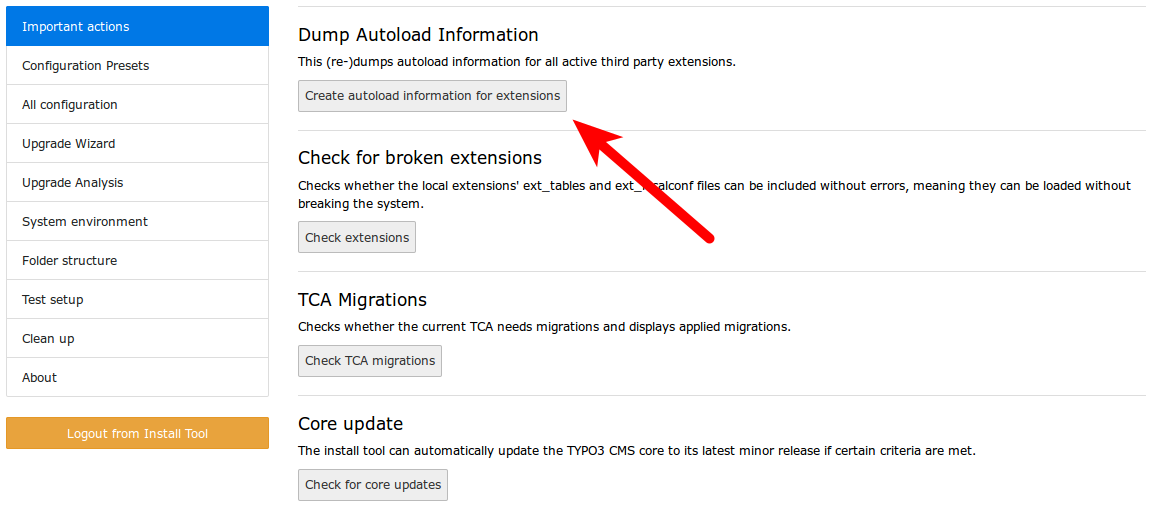
\includegraphics[width=0.8\linewidth]{BackendUserInterface/78222.png}
	\end{figure}

\end{frame}

% ------------------------------------------------------------------------------
% LTXE-SLIDE-START
% LTXE-SLIDE-UID:		bfa12ba2-5527d475-70d937b6-ab220da9
% LTXE-SLIDE-ORIGIN:	5a194e82-8eac7f1b-ef2730da-61d781b2 English
% LTXE-SLIDE-TITLE:		Install Tool: TCA Migration Messages
% LTXE-SLIDE-REFERENCE:	#77799: Display TCA migration messages in Install Tool
% ------------------------------------------------------------------------------

\begin{frame}[fragile]
	\frametitle{Backend User Interface}
	\framesubtitle{Install Tool: TCA-Migration-Nachrichten}

	Im Install Tool kann man nun die TCA-Migration-Nachrichten überprüfen.

	\begin{figure}
		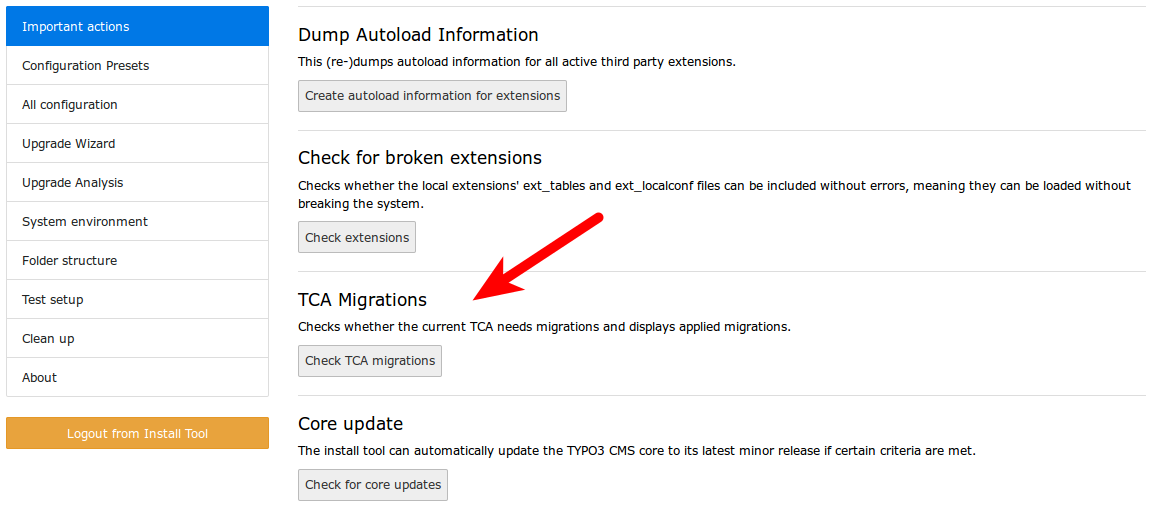
\includegraphics[width=0.8\linewidth]{BackendUserInterface/77799.png}
	\end{figure}

\end{frame}

% ------------------------------------------------------------------------------
% LTXE-SLIDE-START
% LTXE-SLIDE-UID:		25924296-8a3b51a3-a8230fa2-c20a698c
% LTXE-SLIDE-ORIGIN:	1e11eae3-872938ec-9612c092-444c408a English
% LTXE-SLIDE-TITLE:		sys_language records are sortable now
% LTXE-SLIDE-REFERENCE:	#77652: Make sys_language records sortable
% ------------------------------------------------------------------------------

\begin{frame}[fragile]
	\frametitle{In-Depth Changes}
	\framesubtitle{\texttt{sys\_language} Records}

	Um die Usability zu erhöhen, können nun \texttt{sys\_language} Einträge manuell sortiert werden.

	\begin{figure}
		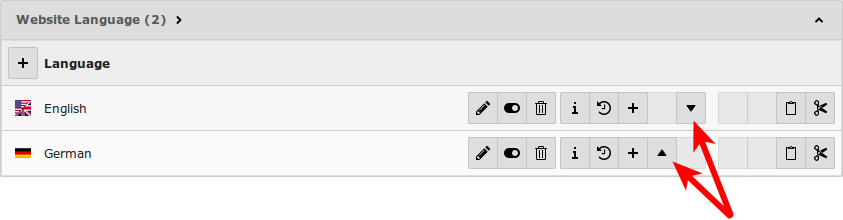
\includegraphics[width=0.8\linewidth]{BackendUserInterface/77652.png}
	\end{figure}

\end{frame}

% ------------------------------------------------------------------------------
% LTXE-SLIDE-START
% LTXE-SLIDE-UID:		eb3aeb2d-26917adf-8b7a0e98-b417e33b
% LTXE-SLIDE-ORIGIN:	a82823ff-94b9520f-5e6d6056-95f1a797 English
% LTXE-SLIDE-TITLE:		#77668: Hide table listing below group element
% ------------------------------------------------------------------------------

\begin{frame}[fragile]
	\frametitle{TSconfig \& TypoScript}
	\framesubtitle{Table Listing Below Group Element}

	\begin{itemize}

		\item Die TCA-Konfigurations-Einstellung \texttt{disable\_controls} des Typs "group"
			besitzt nun eine neue Einstellung \texttt{allowedTables}, welche den Hinweis zu
			erlaubten Tabellen im Gruppen-Feld versteckt.

	\end{itemize}

	\begin{figure}
		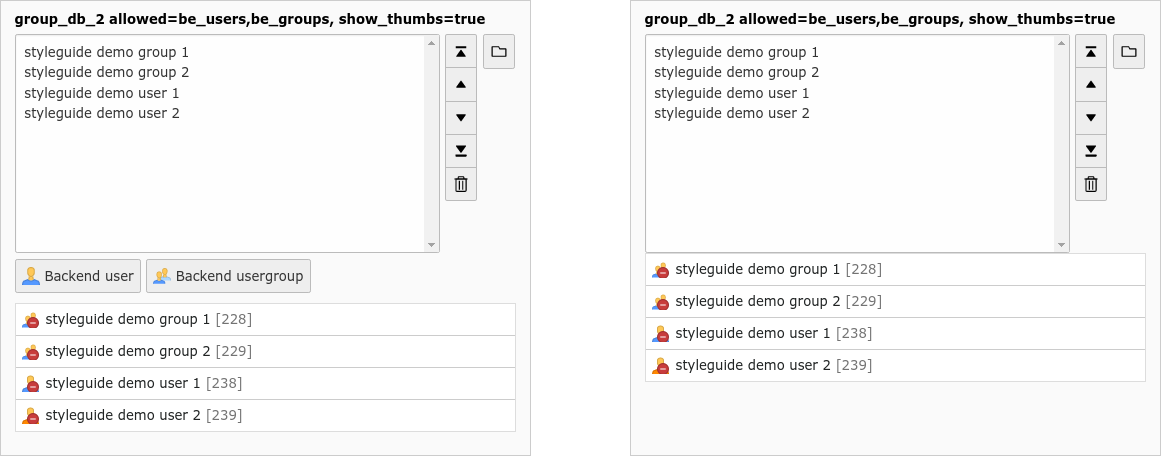
\includegraphics[width=0.85\linewidth]{BackendUserInterface/77668.png}
	\end{figure}

\end{frame}

% ------------------------------------------------------------------------------
